\chapter{Конструкторская часть}
В данном разделе будут реализованы схемы алгоритмов сортировок и будут приведены рассчеты трудоемкостей для этих алгоритмов.

\section{Разработка алгоритмов}
На рисунке \ref{fig:Radix} представлена схема поразрядной сортировки.

На рисунке \ref{fig:Comb} представлена схема сортировки расческой.

На рисунке \ref{fig:Shell} представлена схема сортировки Шелла.

\begin{figure}[h]
	\centering
	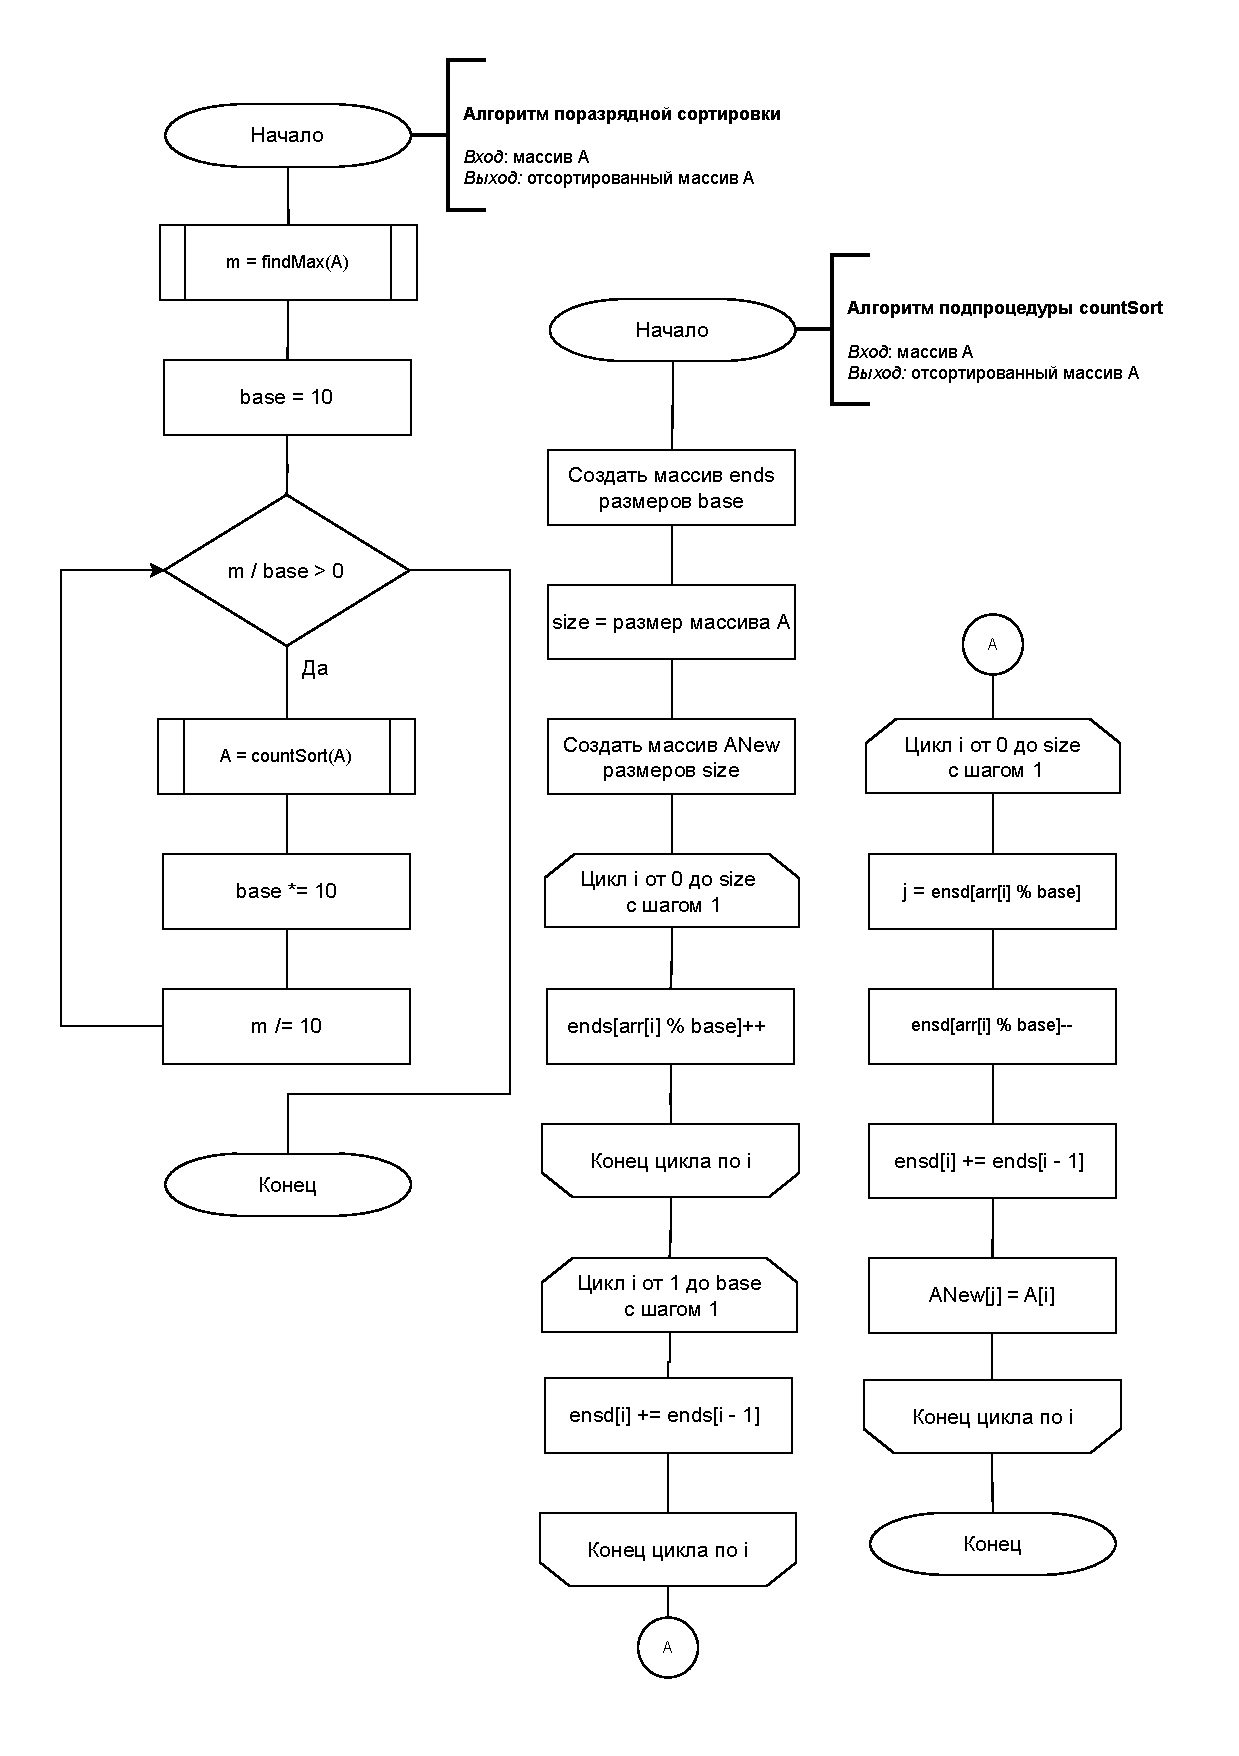
\includegraphics[height=0.9\textheight, page=1]{img/algorithms.pdf}
	\caption{Схема алгоритма поразрядной сортировки}
	\label{fig:Radix}
\end{figure}

\clearpage

\begin{figure}[h]
	\centering
	\includegraphics[height=0.9\textheight, page=2]{img/algorithms.pdf}
	\caption{Схема алгоритма сортировки расческой}
	\label{fig:Comb}
\end{figure}

\clearpage

\begin{figure}[h]
	\centering
	\includegraphics[height=0.9\textheight, page=3]{img/algorithms.pdf}
	\caption{Схема алгоритма сортировки Шелла}
	\label{fig:Shell}
\end{figure}

\clearpage

\section{Модель вычислений для проведения оценки трудоемкости алгоритмов}
Для последующего вычисления трудоемкости необходимо ввести модель вычислений:

\begin{enumerate}
	\item операции из списка \ref{eq:operations1} имеют трудоемкость \textbf{1};
	\begin{equation}
		\label{eq:operations1}
		\begin{gathered}
			+, -, =, +=, -=, ==, !=, <, >, <=, >=, [], \\ ++, --, \&\&, >>, <<, ||, \&, |
		\end{gathered}
	\end{equation}
	\item операции из списка \ref{eq:operations2} имеют трудоемкость \textbf{2};
	\begin{equation}
		\label{eq:operations2}
		*, /, \%, *=, /=, \%=
	\end{equation}
	\item трудоемкость условного оператора \texttt{if условие then A else B} рассчитывается как \ref{eq:if};
	\begin{equation}
		\label{eq:if}
		f_{if} = f_{\text{условия}} + 
		\begin{cases}
			f_{A}, & \text{в случае выполнеия условия,}\\
			f_{B}, & \text{иначе}.
		\end{cases}
	\end{equation}
	\item трудоемкость цикла рассчитывается как \ref{eq:for}
	\begin{equation}
		\label{eq:for}
		\begin{gathered}
			f_{for} = f_{\text{инициализация}} + f_{\text{сравнения}} + M_{\text{итераций}} \cdot (f_{\text{тело}} +\\
			+ f_{\text{инкремент}} + f_{\text{сравнения}});
		\end{gathered}
	\end{equation}
	\item трудоемкость вызова функции равна 0.
\end{enumerate}

\section{Трудоемкость алгоритмов}
В следующих частях будут приведены рассчеты трудоемкостей алгоритмов сортировок.

Трудоемкость обмена элементов местами равна 5.

Пусть размер сортируемого массива~--- $size$.

\subsection*{Поразрядная сортировка}
Трудоемкость алгоритма поразрядной сортировки равна:
\begin{equation}
	f_{radix} = 1 + 1 + m \cdot (1 + 1 + f_{count}).
\end{equation}
где $m$~--- число разрядов в максимальном числе;
$f_{count}$~--- трудоемкость сортировки разрядов подсчетом.

Трудоемкость $f_count$ равна:
\begin{equation}
	f_{count} = 1 + 2 + size \cdot (2 + 4) + 2 + 9 \cdot(2 + 4) + 2 + size \cdot (2 + 9) = 17 \cdot size + 61.
\end{equation}

Итоговая трудоемкость поразрядной сортировки равна:
\begin{equation}
	f_{radix} = 2 + m \cdot (17 \cdot size + 61) = 2 + 17 \cdot size \cdot m + 61 \cdot m \approx O(m \cdot size).
\end{equation}

\subsection*{Сортировка расческой}
Трудоемкость алгоритма сортировки расческой равна:
\begin{equation}
	f_{comb} = 5 + f_{for_{1}} \cdot f_{for_{2}}.
\end{equation}
Трудоемкость внешнего цикла равна:
\begin{equation}
	f_{for_{1}} = 1 + log_{koef}{size} \cdot(3 + f_{for_{2}}) 
\end{equation}
Трудоемкость внутреннего цикла равна:

\textbf{Лучший случай:} когда элементы массива уже отсортированы или практически (т. е. количество перемещений мало).
\begin{equation}
	f_{for_{2}} = 2 + size \cdot(2 + 4) =  2 + size \cdot 6 \approx O(size).
\end{equation}

Итоговая трудоемкость для лучшего случая равна: 
\begin{equation}
	f_{comb} = O(size \cdot log_{koef}{size}).
\end{equation}

\textbf{Худший случай:} когда элементы массива расположены в обратном порядке.
\begin{equation}
	f_{for_{2}} = 2 + size \cdot(2 + 4 + size) =  2 + 2 \cdot size + size^2 \approx O(size^2).
\end{equation}

Итоговая трудоемкость для худшего случая равнв: 
\begin{equation}
	f_comb = O(size^2).
\end{equation}

\subsection*{Сортировка Шелла}
Трудоемкость алгоритма сортировки Шелла равна:
\begin{equation}
	f_shell = 3 + f_{for_{1}} \cdot f_{for_{2}}.
\end{equation}
Трудоемкость внешнего цикла равна:
\begin{equation}
	f_{for_{1}} = 2 + log_2{size} \ cdot (2 + f_{for_{2}}) \approx O(log_2{size}) .
\end{equation}
Трудоемкость внутреннего цикла равна:
\begin{equation}
	f_{for_{2}} = 2 + \frac{size}{n} \cdot (2 + 4 + f_{swap}) \approx O(\frac{size}{n}), 
\end{equation}
где $n$ изменяется во внешнем цикле.

\textbf{Лучший случай:} когда элементы массива уже отсортированы или практически (т. е. количество перемещений мало).
\begin{equation}
	f_{swap} = O(1), 
\end{equation}

Итоговая трудоемкость для лучшего случая равна: 
\begin{equation}
	f_{shell} = O(log_2{size} \cdot size).
\end{equation}

\textbf{Худший случай:} когда элементы массива расположены в обратном порядке.
\begin{equation}
	f_{for_{3}} = 6 + size \cdot (6 + 5 + size) = 6 + 11 \cdot size + size^2 \approx O(size^2).
\end{equation}

Итоговая трудоемкость для худшего случая равнв: 
\begin{equation}
	f_{shell} = O(size^2).
\end{equation}

\section*{Вывод}
В данном разделе на основе теоретических данных, полученных в аналитическом разделе, были построены схемы алгоритмов сортировок. 
Оценены трудоемкости в лучшем и худшем случаях. 

Трудоемкость сортировки расческой и Шелла в лучшем случае: $O(size \cdot log_2{size})$; в худшем: $O(size^2)$.

Трудоемкость поразрядной сортировки в большинстве случаев рвна $O(size \cdot m)$.









